\documentclass{article}
\usepackage[colorlinks=true,linkcolor=black,urlcolor=blue]{hyperref} %% links
\usepackage{graphicx}

\title{SETAP}
\begin{document}
\maketitle
Bradley Edmondson - UP2015336,
Imran Mulindwa - UP2071998,
Hassan Alghamdi - UP2092245,
Fahad Al Rakan - UP2092234,
Jude Whiting - UP2065429,

\tableofcontents
\newpage
\section{Introduction}%
\label{sec:intro}
We are making a top down 2d survival game.

\section{Problem Specification}%
\label{sec:problem}
\subsection{Eliciting requirements}%
\label{subsec:reqs}
To elicit requirements we have used interviews and questionnaires. Our target age group is that of
people 15 years to 30 years old. This is because this reflects the demographic
of people who play games within this genre. Of course while people outside of
this group can play the game. The likelyhood of them doing so is lesser

Our interviews were a discussion with 9 people. these ranged in age from 15 to
21. People had the abiliy to discuss within the answers and expand on their
views even if it was not fully related.
our questions were
\begin{enumerate}
	\item What kind of games do you play?
	\item What are your thoughts on open-world games?
	\item What platform do you play games on?
	\item If you play games for an end goal, what kind of end goal are you looking for?
	\item Are you more into singleplayer or multiplayer games?
	\item What features do you like in the games you play?
\end{enumerate}
\subsection{Interviews}%
\label{subsec:interviews}
In this section I include the data we got from interviews.
\subsubsection*{Age and Gender}
\begin{itemize}
	\item P1: 20, male
	\item P2: 19, female
	\item P3: 19, male
	\item P4: 20, male
	\item P5: 19, female
	\item P6: 20, Male
	\item P7: 19, Male
	\item P8: 20, Male
\end{itemize}

\subsubsection*{What platforms do you play on?}
\begin{itemize}
	\item P6: PlayStation, PC
	\item P7: PlayStation
	\item P8: PlayStation
\end{itemize}

\subsubsection*{What kind of games do you play?}
\begin{itemize}
	\item P1: Fifa, Call of Duty
	\item P2: Life simulation, Roleplay, Building eg Sims, Minecraft, Stardew Valley
	\item P3: Single player action adventure games, eg God of War, Resident Evil
	\item P4: Party games, Mario Kart, Overcooked, Roguelikes
	\item P5: Minecraft, Sims, Dead by Daylight, story based indie games
	\item P6: Single player, Open-world e.g. God of War, Grand Theft Auto, Darksiders
	\item P7: Sandbox, Action and Adventure
	\item P8: Sports
\end{itemize}

\subsubsection*{What features do you like in the games you currently play?}
\begin{itemize}
	\item P1: Receiving strong rewards for doing well or getting lucky
	\item P2: Building, character customisation
	\item P3: Good story, world design, rpg system e.g. armour and stat customisation
	\item P4: It’s just lots of fun when  you’re in the same room as someone playing a game together, with lots of excitement and emotions.
	\item P5: The story, character customisation
	\item P6: Hack ‘n’ slash, variety of enemies, quicktime events, range of difficulty
	\item P7: Graphics design
	\item P8: User able to make decisions regarding the game
\end{itemize}

\subsubsection*{What are your thoughts on open-world games?}
\begin{itemize}
	\item P1: Played them when I was younger,I played minecraft and terraria
	\item P2: Like them, think they're fun
	\item P3: Can be pretty good, sometimes lack detail
\end{itemize}

\subsubsection*{How difficult do you like your games to be?}
\begin{itemize}
	\item P1: Hard, because you get a stronger sense of accomplishment when you overcome the challenge
	\item P2: On the easier side
	\item P3: A good balance (fairly challenging)
	\item P4: A bit hard - hard
	\item P5: Challenging
	\item P6: Very hard
\end{itemize}

\subsubsection*{Would you like it if a game heavily punished you for making a mistake?}
\begin{itemize}
	\item P1: Completely restarting when you die is too much, keeping some items and abilities is fine
	\item P2: No, roguelike style still too much
	\item P3: As long as you don’t get killed for a BS reason, then losing everything and restarting is fine.
	\item P4: Keeping some items and abilities when you die seems fair
	\item P6: Yes, it makes you work harder and develop a mental strategy for each fight
	\item P7: No because all of your achievements playing the game will be lost
	\item P8: No because you will have to replay the game all of over again
\end{itemize}

\subsection{Requirements}%
\label{subsec:ureqs}
These requirements are garnered from our interviews \ref{subsec:interviews}. Our main line is our user
requirements with each of them broken down into a set of system requirements.

These are ordered in the priority of these tasks. The first ones being the most
important, the latter being the least. This is both for the user requirements
and the system requirements within them.

%% This level of detail good
%% TODO: update all of them to reflect this kind of detail
\paragraph{Users should be able to play the game on multiple operating systems}
\begin{itemize}
	\item Users with different operating systems like windows, Linux will gain access to the features that are provided by the application
	\item The system should be easily installable on platforms that it is compatible from different operating systems e.g., windows, Linux
	\item When the system is in use, it shouldn’t take more than 3 minutes to load data and should respond to gameplay commands such as movement.
	\item Users who have different platforms other than Windows or Linux, the system may not be accessible.
	\item The game should not crash, instead the error should be handled and an error message shown to the user.
	\item Users should find the system intuitive to use. Using long standard practices from the game industry such as movement commands and so on.
	\item The system should not take more than 10 seconds to launch the game.
\end{itemize}

\paragraph{Users should be able to explore a procedurally generated map.}
\begin{itemize}
	\item The map size will be 100 x 100 and include 10,000 tiles in total.
	\item Each tile should be able to carry 1 item and character (user or NPC).
	\item The player will move by moving from tile to tile.
	\item Users will spawn in the middle of the map at point (50, 50).
	\item The map will be modelled as an object.
\end{itemize}

\paragraph{Users should be able to interact with NPCs.}
\begin{itemize}
	\item Interactions will be both hostile and passive depending on the type of NPC.
	\item Each NPC will be modelled as an object that interacts with the user.
	\item NPCs will drop items when killed, which the user should be able to collect.
	\item There will be passive NPCs that can sell you stuff using a bartering system.
\end{itemize}

\paragraph{Users should be able to save their progress into a save file.}
\begin{itemize}
	\item Will produce a save file for storing, maintaining and accessing data
	\item The file should store the world map as a 2D array.
	\item The file should store the user’s current inventory and that of any chests they have placed.
	\item The file should store the user’s position and the position of any spawned NPCs or items.
	\item The file should store the user’s current points acquired and stats (health, speed etc.).
	\item A save file for the current game will be saved up to every 10 minutes.
\end{itemize}

\paragraph{Users should be able to collect resources.}
\begin{itemize}
	\item Resources will be represented as different assets on the games stage.
	\item Users will have to manually collect items, by pressing the letter e key.
	\item Each resource will add to the point system.
	\item They will be modelled internally as objects.
	\item Rarity will be given as an attribute to give the object its points value.
\end{itemize}

\paragraph{Users should be able to generate points.}
\begin{itemize}
	\item Points will feed into a point system which will generate highscores.
	\item Users will gather points from collecting resources, killing NPCs, crafting items etc.
	\item Points will improve a user's stats (health, speed etc.)
	\item Each point collected must be shown to the user within 2 seconds.
	\item The system should provide users of the total points collected on each session.
	\item The system shall measure the time of each session and show it at the end of the session.
\end{itemize}

\paragraph{Users should be able to use weapons.}
\begin{itemize}
	\item Weapons will be found or crafted by the user.
	\item Weapons will deal a set amount of damage.
	\item Different weapons should deal different amounts of damage.
\end{itemize}

\paragraph{Users should be able to use a simple crafting system.}
\begin{itemize}
	\item Users will craft new items using items from their inventory that they have collected.
	\item Crafting recipes will show up depending on what’s in a user's inventory.
	\item An item’s rarity should change when item’s of different rarities are crafted together.
\end{itemize}

\paragraph{Users should be able to play together using local multiplayer.}
\begin{itemize}
	\item A game should be able to be set as joinable or not when it is started.
	\item Up to 4 users should be able to connect to the same game.
	\item The system should be scalable enough to support multiple users, on the same network, at the same time while maintaining optimal performance outside of constraints we cannot control such as users hardware and networks.
	\item Users should identify during multiplayer games, with a name they provide before a connection is created.
	\item The game should not crash under the pressure of many users playing.
	\item TODO: mention protocol
\end{itemize}

\paragraph{Users should be able to use a chest system.}
\begin{itemize}
	\item Chests should be able to be crafted and placed into the world by users.
	\item A user should be able to view all the items that are in a chest.
	\item Items will be able to move between the user's inventory and the chest.
\end{itemize}

\paragraph{Users should be able to select difficulty}
\begin{itemize}
	\item Enemies will be stronger the harder the difficulty is
	\item Resources may be harder to find
	\item Crafting may require more resources
	\item Difficulty should be selected when a new game is created.
\end{itemize}

\paragraph{The System should be accessible}
\begin{itemize}
	\item The application will have features that match the geographical location of the users i.e. languages, time zones. This will give the users opportunity to choose which geographical location is the best to use
	\item The game must be engaging, with users responding back telling us how they enjoyed what they can and can’t do.
	\item The game must support different colour spectrums to support colour
	      blind people
	\item This will be activated in a small options menu
\end{itemize}

\section{Design}%
\label{sec:deign}
%% TODO: add in user interaction diagram.
%% 5 senarios
%% diagrams not needed
%% TODO: add in architecture diagram
\subsection{Use cases}%
\label{subsec:cases}
\subsubsection{Use Case: Enter Username}
\begin{itemize}
	\item Actor: User
	\item Description: When playing on a multiplayer game a user attempts to enter a username to go by on the server.
	\item Pre-Condition: User has attempted to create or join a multiplayer game.
	\item Post-Condition: The user joins the game with their entered username.
	\item Data: Input: User’s username / Output: Game loads/Error message
	\item Valid Case: User loads an input text box and a message asking them to input a username. The user inputs a username and presses enter. The user is then sent to the game loading screen.
	\item Error Case: Username not valid: If the user name is invalid an error message will be shown to the user and they will be sent back to the enter username screen.

\end{itemize}

\subsubsection{Use Case: New Game}
\begin{itemize}
	\item Actor: User
	\item Description: A user attempts to create a new game.
	\item Pre-Condition: User has loaded up the game and has selected ‘New Game’.
	\item Post-Condition: The game has been created and the user is loading into the game.
	\item Data: Input: Game name / Output: Game loads/Error message
	\item Valid Case: User loads an input box to enter a name for that game to be saved under. The user enters a name and presses enter. The user is then sent to the game loading screen.
	\item Error Case: Name is invalid: If the name is invalid an error message will be shown to the user and they will be sent back to the enter name screen.

\end{itemize}

\subsubsection{Use Case: Load Game}
\begin{itemize}
	\item Actor: User
	\item Description: A user attempts to load a previously created and saved game.
	\item Pre-Condition: User has loaded up the game and has selected ‘Load Game’.
	\item Post-Condition: The user is loaded into the game at the point of where they last saved that game.
	\item Data: Input: Selecting a game to load / Output: Game Loads/Error Message
	\item Valid Case: User has been presented with a list of saved games and chooses the correct one to load. The user is then sent to the game loading screen.
	\item Error Case: File corruption: A save file could corrupt and then an error message would be sent to the user and they would be sent back to the menu screen.
\end{itemize}
\subsubsection{Use Case: Save Game}
\begin{itemize}
	\item Actor: User
	\item Description: A user attempts to save their current progress in their game.
	\item Pre-Condition: User has clicked the button on the screen titled ‘Save Game’.
	\item Post-Condition: All the data about the current game is stored into a save file, overwriting any previous save data.
	\item Data: Input: Pressing the save button / Output: Success/Error Message
	\item Valid Case: The game freezes while the game saves and then the user is given a success message to say the game has saved. Then the game resumes as usual.
	\item Error Case: Saving was interrupted, the user is given an error message and told to retry. This then resumes the game and the user can retry saving it.
\end{itemize}

\subsubsection{Use Case: Join Game}
\begin{itemize}
	\item Actor: User
	\item Description: A user attempts to join a multiplayer game that another user created.
	\item Pre-Condition: User has loaded up the game and selected ‘Multiplayer’.
	\item Post-Condition: The user is told to enter a username.
	\item Data: Input: Selecting a game to join / Output: Joins game/Error message
	\item Valid Case: The user is taken to the enter username page and once that is completed, successfully loads into the game along with the other players.
	\item Error Case: Network connection error, the user has received a network error and is presented with an error message and told to retry. This then places at the user on the main menu/

\end{itemize}

\subsubsection{Overall Use cases}
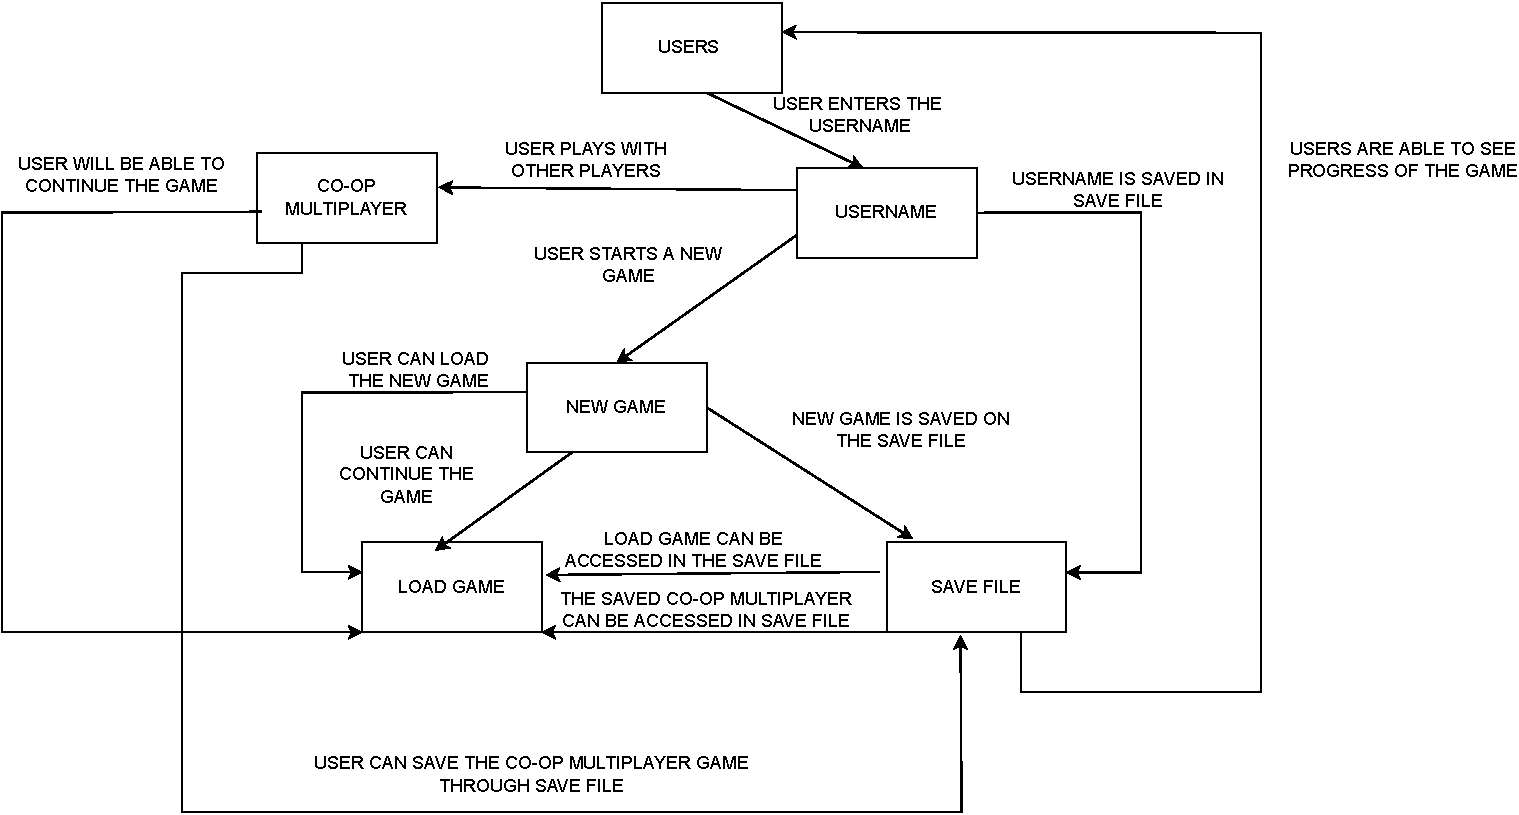
\includegraphics[scale=0.5,page=1]{2DGAME (1)-crop.pdf} \\
Users: This use case is described as people who will be involved in playing the game.
username : This is the procedure that allows users to gain access to the system. When users have entered their username, they will be able to acquire the features of the system like new game, load game etc. in the login, users won't have to re-enter their usernames since they are saved in the save file
New Game: This use case allows users to start the game from the beginning therefore anyone who plays the 2D game from the beginning will be able to understand how the game works quickly. Users will be able to continue the game through load game and the game will always  be saved in the save file
Load Game: This use case will allow users to continue the game where they have previously left off. So, users will have the opportunity to not start the game again. The load game will be got from the save and accessed
Save File: This use case allows the user to save the whole content of data through gameplay of the user. It also shows where the user stopped playing within the game. The save file will also contain the co-op multiplayer
Co-op multiplayer: users will be able to play with other users and always continue where they have left off from the load game when they save their game in the save file. Once, they continue the game they will not lose their previous achievements except when they didn’t save the game

\subsection{Architecture}%
\label{subsec:arch}
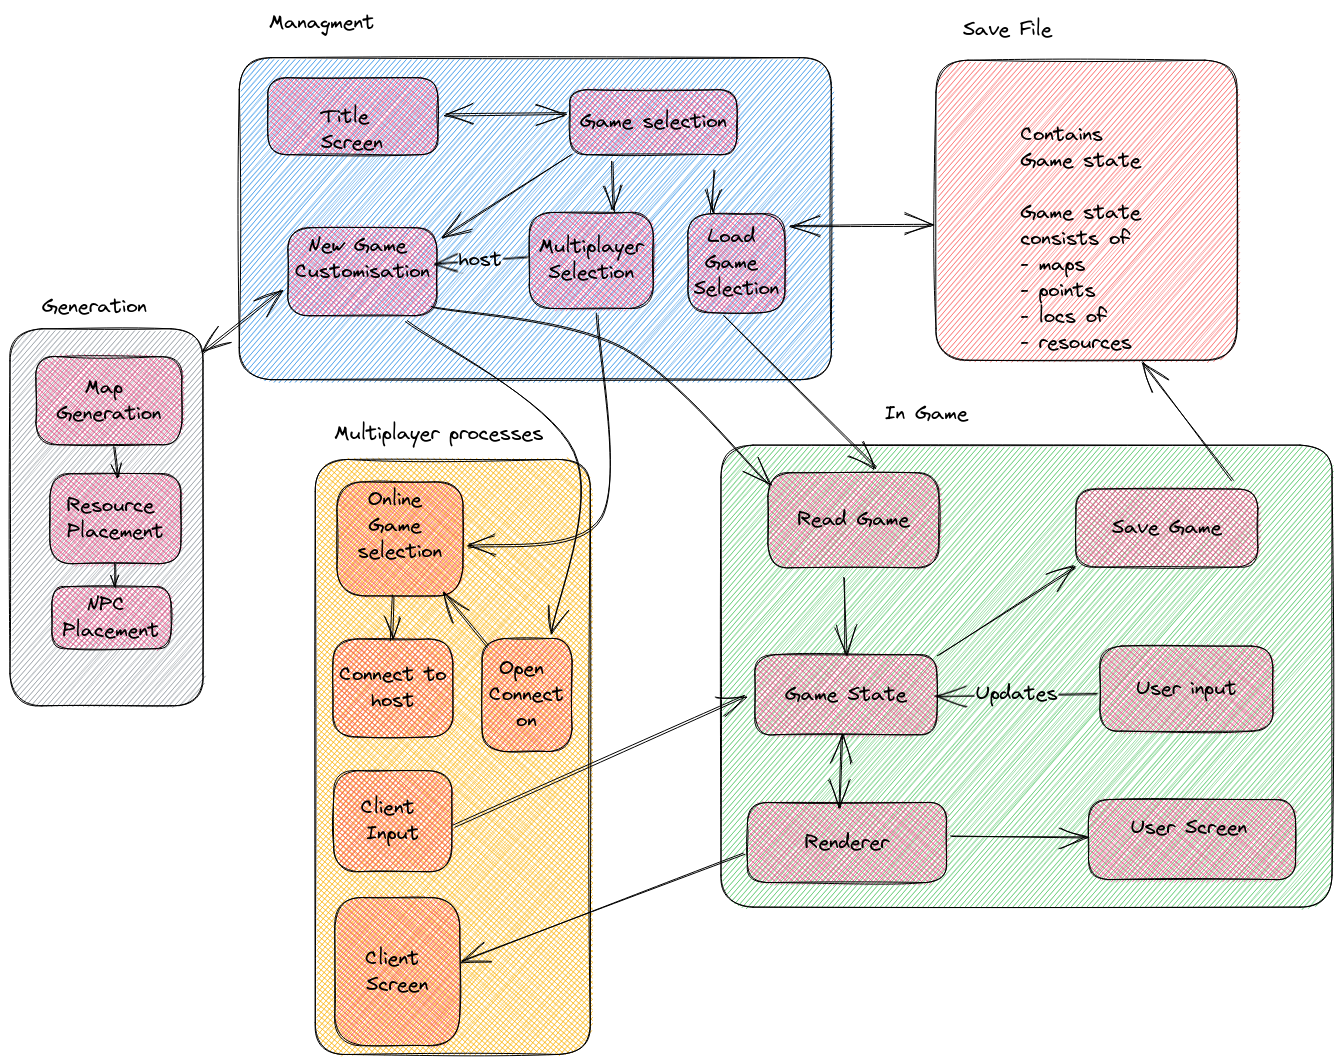
\includegraphics[scale=0.2]{architecture.png} \\
Our architecture consists of 5 main parts.
These include
\begin{itemize}
	\item The managment of the game: section which manages the loading of games. It contains the
	      selction menus and guides the users towards creating or loading a new
	      game
	\item Game generation: This creates the datastructures that will be read by
	      the game state which then runs the game
	\item The game itself which will read the game save into the game state,
	      as well as update the game state based on user input
	      this gets passed into the renderer which renders it to the user screen
	\item the save file which stores the data, this will perodically be re
	      saved.
	\item The multiplayer processing, this encapsulates all of the
	      multiplayer game processing.
\end{itemize}
\section{Implementation}%
\label{sec:impl}
Our implementation will be completed in the Lua language and the love game
engine. We chose these tools as:
\begin{itemize}
	\item Lua is a small and simple language to learn. Being similar to python while
	      having many differing uses from python
	\item Love is a simple game engine, focusing in on 2d game development and
	      having a small and simple interface while still being able to express
	      larger and more complex games
\end{itemize}

%% TODO: add in workflow
We will be using git and github for our code management.
\begin{itemize}
	\item  Issues will be created to discuss features in implementation
	\item Pull requests are used to implement and test features
\end{itemize}

\section{Testing}%
\label{sec:test}
Testing will mainly consist of unit testing. This allows us to test all of our functions in isolation and check that we do not break compatibility within revisions to each prototype. We will test against our non-functional and functional requirements after every prototype iteration.

The requirements will be individually marked as either completed or missing or will have a description of the level of success if the requirement is only partially met.

We will also test the efficiency of our non-functional requirements where we can, and give a mean average of the time taken to run a function for every prototype to help track efficiency improvements throughout the project cycle.

This will be followed by integration testing and then eventually user testing, where we will ask fellow students to play each iteration of the prototype, and give us feedback on what areas they think need improving and what features they think are missing from the game. This will be important as it will provide us with an unbiased opinion on our project.

\section{Critical Analysis}%
\label{sec:anal}

\subsection{Leadership}%
\label{subsec:leadership}
Our methodology is Scrum. This will involve us assiging tasks into week long
sprints. These tasks will be tracked on a Kanban board hosted on github

We will have the roles of A scrum master and then scrum workers. The former will
delegate the tasks and monitor the progress of these tasks, with how these tasks
progressing being decided at the end of the sprint during our next meeting.

The Scrum master will be voted in during our weekly meetings. Everyone will have
a chance too but people will submit themselves. If no one does then we will
select the next person to not be scrum leader.

\subsection{Monitoring}%
\label{subsec:mon}
All tasks will be out on a monitoring board with a SCRUM Master monitoring progress throughout the week
Tasks are assigned at the beginning of each week.
As tasks are finished they will be move into a different section of the monitoring board
If a task is not finished during a sprint, then either more people will be assigned to it, it will get continued over to the next week or it will be reassigned to someone else

\subsection{Conflict resolution}%
\label{subsec:cres}

If a conflict of opinion comes into being. Then we will discuss this first in
our online communication channels.
If it does not resolve there then we will move this to a meeting, after
discussion with the entire group we will vote on it. A majority vote will be
taken.
If that fails to resolve the issue we will seek mediation from a third party

\subsubsection{Case study}
When deciding for this project we had mulitple projects we wanted to do.
This was not completed during our first session and we had a split between an
image sharing app and this 2d game.
We discussed this over our discord server and decided this would be better to
discuss in person.
During this in person meeting we wrote up the pros and cons of each, listing out
the technologies and the interesting sections of the problems. and finally came
to a vote. This process of multiple discussions was simple yet effective

\section{Contributions}%
\label{sec:contrib}
\begin{tabular}{c | c}
	UP Number & contribution    \\
	\hline                      \\
	UP2015336 & equal           \\
	UP2071998 & equal           \\
	UP2092245 & equal           \\
	UP2092234 & equal           \\
	UP2065429 & equal           \\
	UP928651  & no contribution
\end{tabular}

\end{document}
